%!TEX root = main.tex
% \section{Solution}
% \label{sec:solution}
\section{SageSched Design}
\label{sec:design}

\begin{figure}
    \centering
    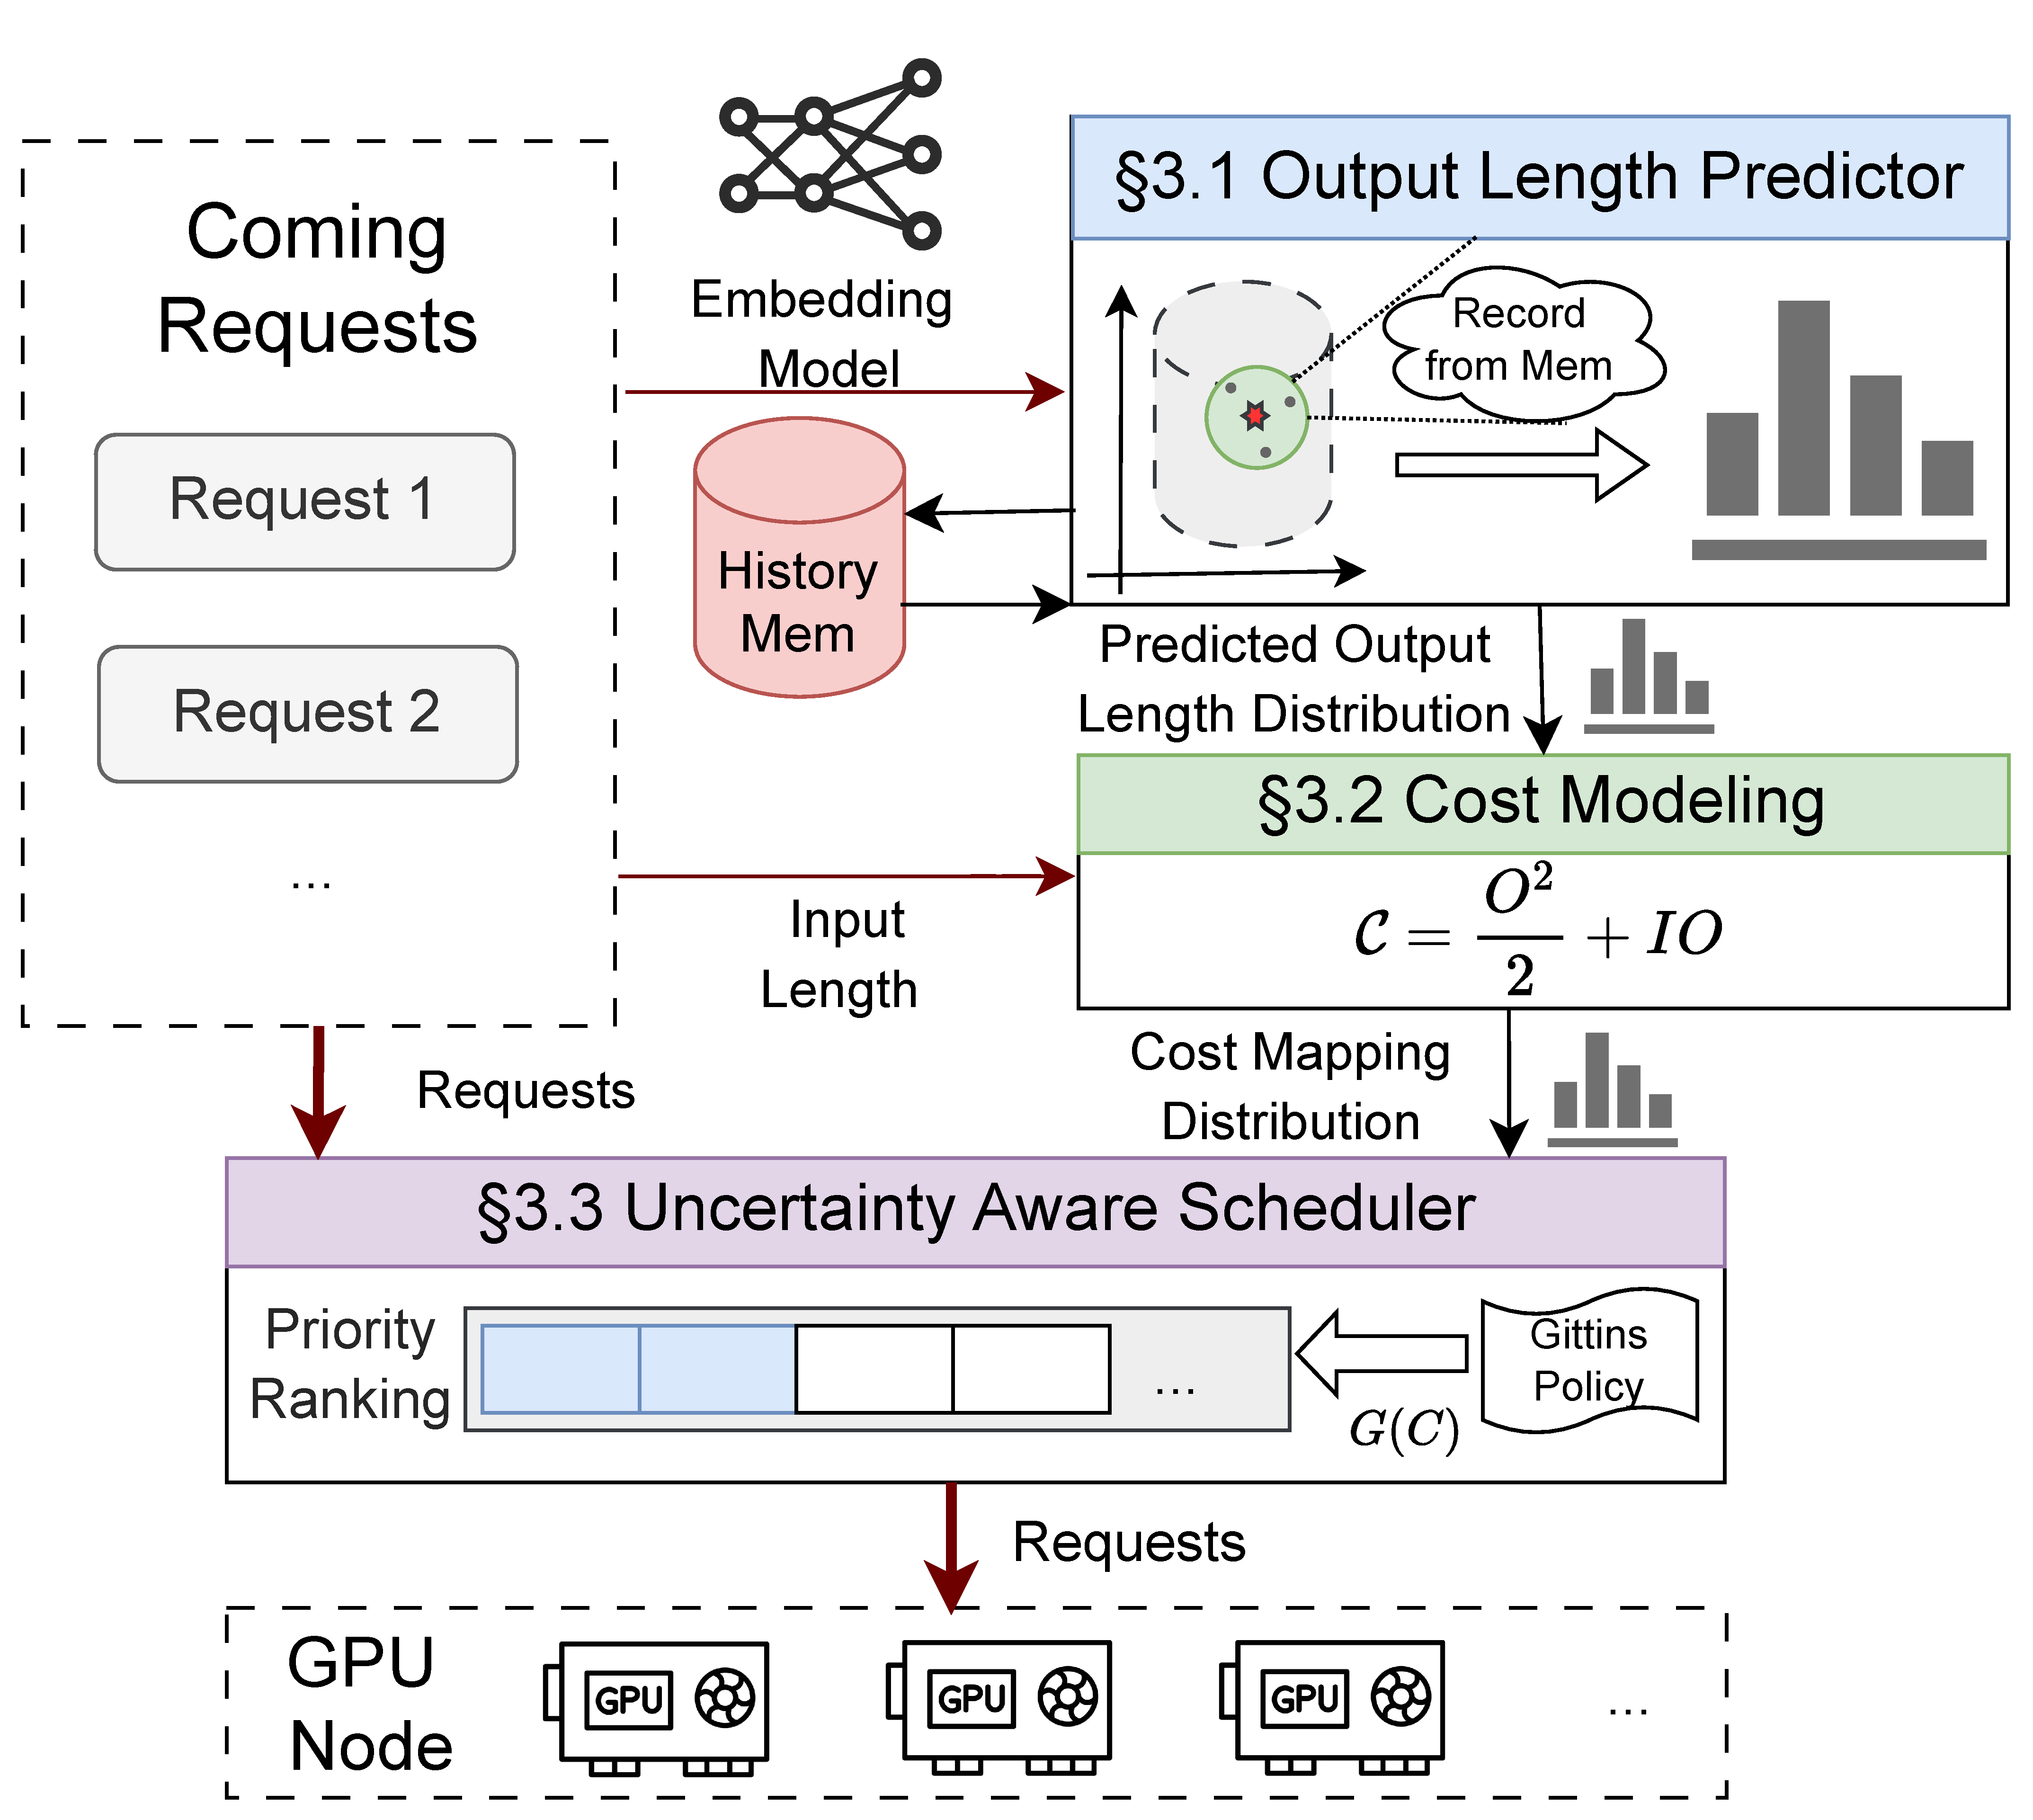
\includegraphics[width=0.8\linewidth]{figures/overview_new.pdf}
    \caption{Overview of \oursched workflow.}
    \label{fig:overview}
\end{figure}

%\phm{Overview.} 
In this paper, we design \oursched, a novel LLM scheduler that, by properly handling dynamicity uncertainty and hybridity, attains efficient TTLT performance. 
The overall workflow of \oursched is elaborated in Fig.~\ref{fig:overview}.
For each incoming LLM inference request, \oursched first predicts its output-length distribution with a light-weight yet also accurate predictor (Sec.~\ref{subsec:predictor}).
It then quantifies the overall service cost of that request based on the predicted output length, with both the memory and compute resources considered (Sec.~\ref{subsec:cost}).
Finally, \oursched employs an uncertainty-aware scheduling algorithm to determine the runtime request queuing order, which can yield the optimal efficiency (Sec.~\ref{subsec:gittins}). 


%\subsection{Training-free Output-length Prediction
\subsection{Semantic-aware History-based Predictor}
%Semantic-Aware Predictor \chen{more concise}}
\label{subsec:predictor}


As elaborated in Sec.~\ref{subsec:limitations}, given the built-in uncertainty of LLM decoding process, a truly accurate prediction method must yield a \emph{distribution} rather than a \emph{number} when depicting the predicted output token length.
In that regard, a straightforward solution is to customize the output-projection layers in existing prediction models (e.g., DistillBert~\cite{distilbert_docs}) for distribution prediction; such a customized model essentially seeks to---given the semantic input prompt---directly \emph{approximate} the ultimate generation effect. % with a smaller-size model.
%, which we call \emph{direct generation-emulating prediction}.
Yet, maintaining such a prediction model is still \emph{costly} (due to the training overheads) and \emph{inaccurate} (due to the complexity to approximate the inference effect).

In fact, given an inference prompt, we find its output length should be better predicted by \emph{referring to similar requests in the recent history}---instead of by directly emulating the inner generation process with a fine-tuned model.
Given the complexity of auto-regressive generation, it would be much easier to \emph{evaluate prompt similarity} than to \emph{directly emulate the generation effect}. 
Meanwhile, existing works~\cite{gong2025past} have revealed that, \emph{the overall distributions of request output length within adjacent sliding time windows are relatively stable}, indicating high reference value of the recent serving history. %potential to make history-based prediction.
Therefore, by selecting the past requests with a similar prompt, we can potentially make \emph{easier-yet-more-accurate} demand prediction. 


\begin{figure}[t]
    \centering
    \subfigure[Prompt-1 sampled from the \emph{Alpaca} dataset]{
        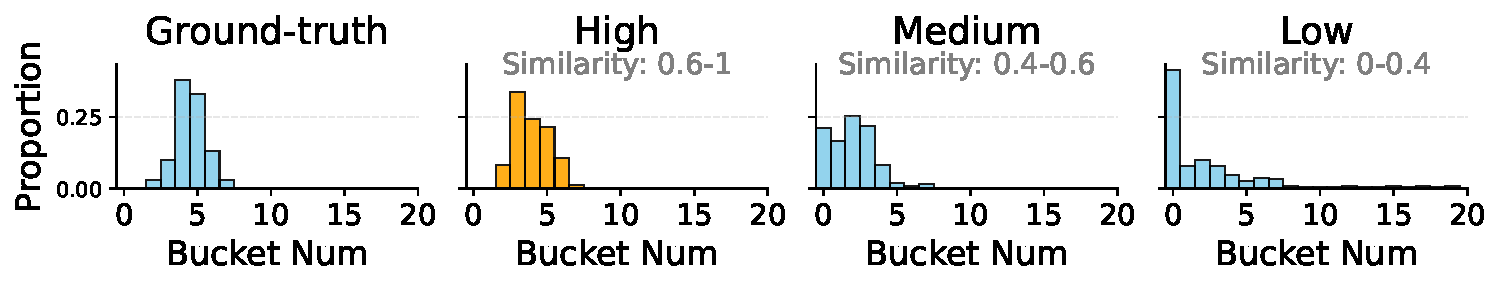
\includegraphics[width=0.9\linewidth]{figures/all_distributions_sample_39.pdf}
        \label{fig:correlation-1}
    }
    \hfill
    \subfigure[Prompt-2 sampled from the \emph{Write} dataset]{
        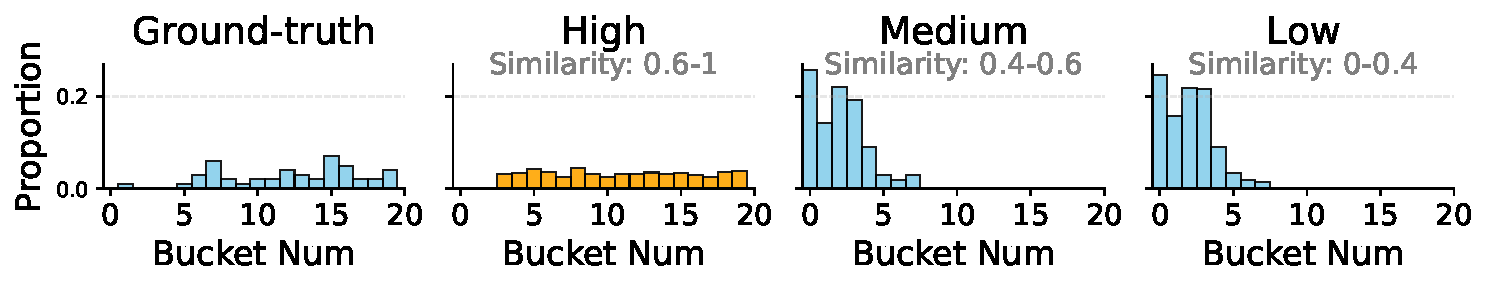
\includegraphics[width=0.9\linewidth]{figures/all_distributions_sample_57.pdf}
        \label{fig:correlation-2}
    }
    \caption{Output-length distribution of a request can be better approximated by historical requests with a higher prompt similarity.} 
    \label{fig:prompt-correlation}
\end{figure}

To explore, we empirically study the correlation between prompt similarity and output-length similarity. 
We sample two prompts respectively from the Alpaca and Write datasets (elaborated in Sec.~\ref{subsec:problem}). 
For each prompt, we first serve it 100 times, obtaining an output-length distribution as the ground-truth to predict.
Then we classify the historical requests into three categories based on their similarity to the selected prompt; here similarity is quantified as the \emph{cosine similarity} between two requests' prompt embeddings. 
As shown in Fig.~\ref{fig:prompt-correlation}, for each case, there exists a clear correlation between the prompt similarity and the output-length-distribution similarity: the curve shapes of \emph{higher-similarity} buckets are \emph{closer} to the target distribution. 



Given the above analysis, we propose \emph{semantic-aware history-based predictor}, which combines the \emph{prompt contents} with the \emph{historical execution status} to directly predict the output length distribution. 
%Therefore, in designing a cost-efficient and also LLM-generic output-length predictor, we propose a novel method called \emph{indirect analog-ensembling prediction} (as apposed to direct generation-emulating prediction).
Specifically, we record the inference information (prompt contents and output lengths) of recently-served requests.
For each incoming request, we search\footnote{Our history window has a size of 10,000 records and keeps updating in a \emph{FIFO} manner. 
    In cases where the high-similarity requests are insufficient (e.g., in the warming-up phase), we augment the searching set with the requests from public datasets.
    We use the efficient \emph{FAISS IndexFlat}~\cite{faiss_meta} {tool} to perform embedding search, which in general takes {less than 1 ms}.
    %over a short-term history of 10k vectors, retrieving the top-100 most similar records, within several tens of milliseconds. 
    %The query time complexity is $\mathcal{O}(N \cdot d)$ where \(N\) is the number of vectors and \(d\) denotes the embedding dimension.
}
for those requests with a sufficiently-similar prompt (with a similarity threshold defaulted to 0.8), and use their output-length distribution as the prediction result.
Such a method does not require fine-tuning any model, thereby being generally applicable to diverse LLMs; neither does it require emulating the complex generation process.
Therefore, in this way we can make light-weight and also accurate prediction for output-length distribution. %, which is later confirmed by our evaluations in \chen{Sec. X}.



\subsection{Resource-bound-based Cost Modeling}
\label{subsec:cost}

With the above prediction method, we can now obtain the output-length distribution for each upcoming request. 
Nonetheless, as explained in Sec.~\ref{subsec:limitations}, due to demand hybridity, it is deficient to directly use the output token length as the service cost of an LLM request.
In this part we need to find a comprehensive cost-depicting model with both compute and memory resources considered. 

We note that for multi-resource cost modeling, it is crucial to first understand which resource is the true bottleneck, which determines the follow-up cost analysis road-map.  
In reality, an LLM service backend may be either \emph{compute-bound} or \emph{memory bound}---depending on the runtime workload characteristics.
Specifically, in Fig.~\ref{fig:diverse_bounds} we depict\footnote{
In Fig.~\ref{fig:bounds_and_observations}, GPU utilization is estimated by comparing the achieved TFLOPs to the peak TFLOPs, and the CUDA time is measured with \texttt{torch.profiler}.
}
the relationship between compute and memory consumptions for a decode step served atop an H100 GPU with increasing batch size.
We respectively fix the sequence length (including both the input length and the latest output length so far) to 50 and 1000.
Longer sequences tend to be more memory-intensive: when serving short sequences, the GPU utilization is already very high before reaching the memory limit; yet for long sequences, the GPU utilization has not yet ramped up when GPU memory is full.
Note that the service cost on a resource type matters only when that resource becomes the bottleneck. 
We therefore explore how to analyze the LLM service cost respectively in each status. 




\begin{figure}[t]
    \centering
    \subfigure[Relationship between GPU utilization and KVCache occupation as batch size increases.
    %(the instantaneous sequence length of each request is respectively fixed to 50 and 1000).
    ]{
        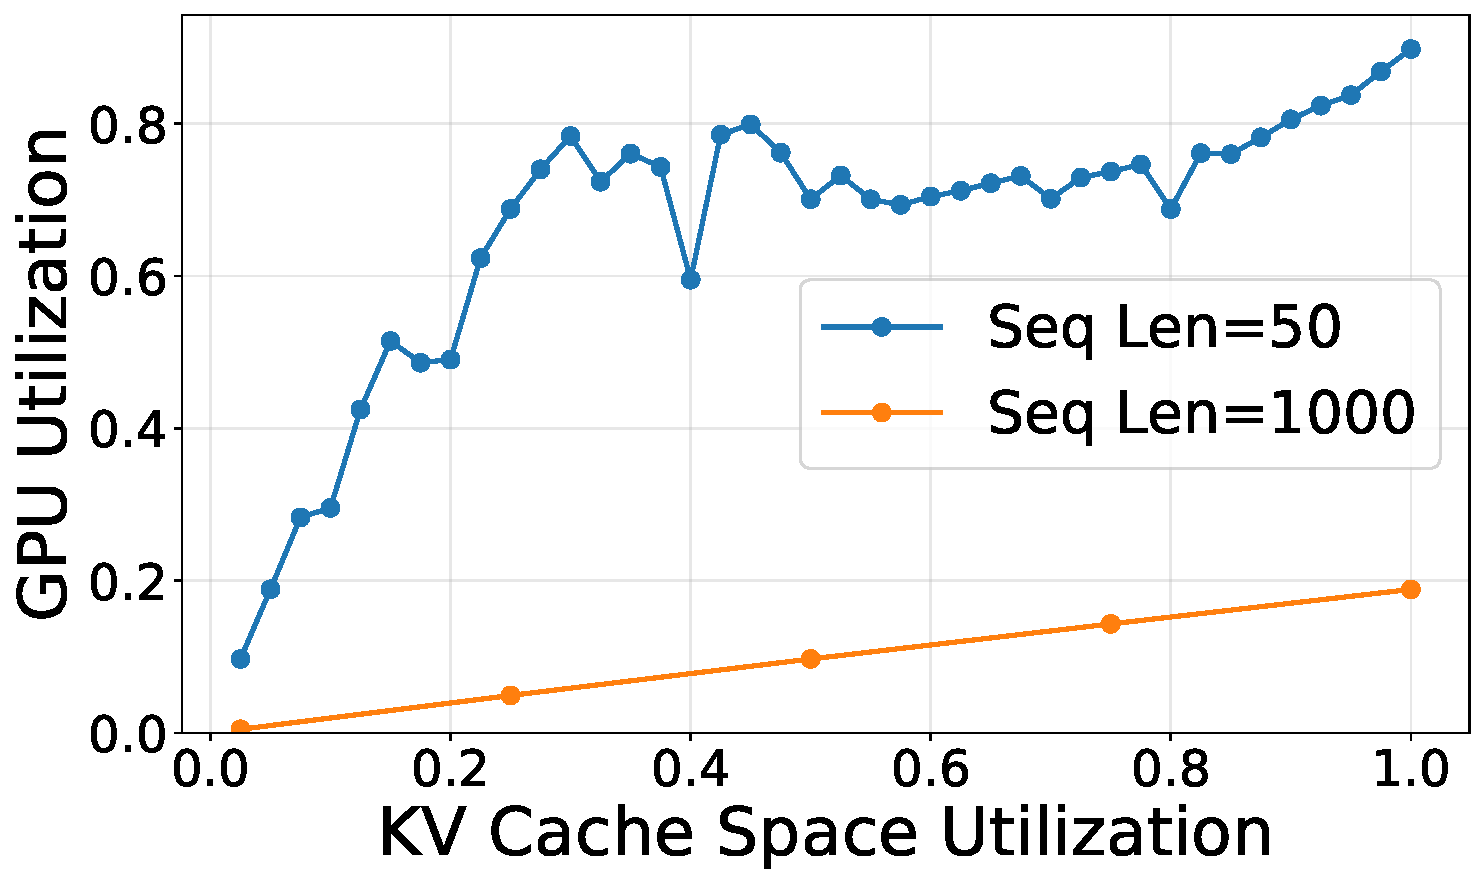
\includegraphics[width=0.45\linewidth]{figures/two_workloads_varying_batch.pdf}
        \label{fig:diverse_bounds}
    }
    \hfill
    \subfigure[Variation of the per-step attention-computation time
    %(including a decomposition of as inference proceeds
    as decoding proceeds.
    ]{
        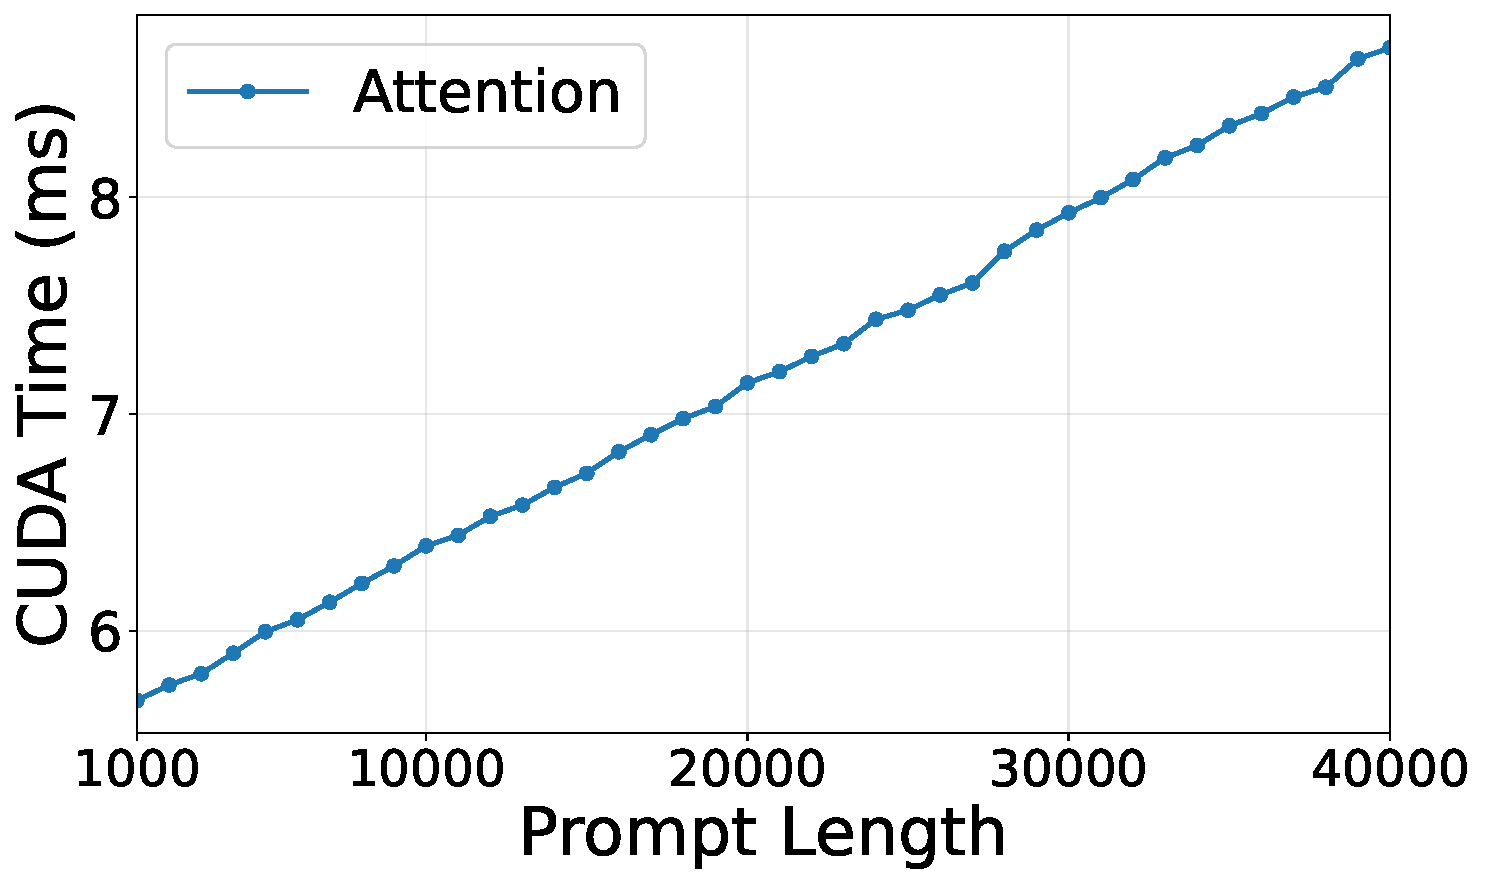
\includegraphics[width=0.45\linewidth]{figures/simple_module_analysis_attention.pdf}
        \label{fig:compute_cost}
    }
    \caption{Measurements on the instantaneous resource bound, as well as the compute cost characteristics in decoding. All measurements are conducted on an H800 GPU with Qwen3-32B model.} %Profiling experiments: (a) LLM serving backends may be either compute or memory bound, and in compute-bound scenarios; (b) the per-step computation cost increases linearly as inference proceeds. Both are conducted on an H800 GPU with Qwen3-32B.}
    \label{fig:bounds_and_observations}
\end{figure}

% \begin{figure}
%     \centering
%     \includegraphics[width=0.7\linewidth]{figures/CostModel.pdf}
%     \caption{The Dynamic Cost Modeling.\chen{repeating with Fig. 3? Consider removal}}
%     \label{fig:modeling}
% \end{figure}


We first focus on inference cost modeling in \emph{memory-bound} status.
In such circumstances, the KVCache occupation of an LLM request is a key factor in cost modeling---less KVCache consumption allows more requests be concurrently served (with low GPU utilization, serving more requests concurrently won't increase the iteration time). 
Therefore, in memory-bound scenarios, we need to primarily consider a request's cumulative KVCache consumption during its inference process.
%That is, let KV(r,t)
That is, let $I$ and $O$ be the input (i.e., prompt) and output token length of an inference, then its total service cost $\mathcal{C}$ can be depicted by $\mathcal{C}_M=\sum_{l=I}^{I+O}l*U_{MT}=(\frac{O^2}{2}+IO)U_{MT}$, where $U_{MT}$ represents the unit \emph{memory-time} product (i.e., the KVCache space occupied by a single token in a single step). 

%$C = \int_{0}^{T} KV(r, t) \, dt$.
%That is, suppose a request $r$ is served for $T$ time and KV(t) is its KVCache occupation at time $$ 

We next turn to the \emph{compute-bound} status. 
In such cases, the KVCache occupation of an LLM inference is not a concern on the service backend, and we only need to quantify its total computation amount over its lifetime.
To that end, in Fig.~\ref{fig:compute_cost}, we measure the per-iteration attention-computation time (a key computing module in Transformers) in different decoding\footnote{
In this paper we focus on resource consumption in \emph{decoding} steps; with the wide adoption of \emph{reasoning LLMs}~\cite{cai2025r}, the decoding phase of an inference often dominates its TTLT.
Moreover, apart from the linear attention-computation time, there also exists a \emph{constant} FFN computation time (as well as some minor time factors like CUDA-lunching delay) that is irrelevant to the sequence length. 
However, the FFN time can be remarkably amortized in long decodes or with large batch sizes (given the GPU GEMM optimizations); so for simplicity we skip it here.  
} steps when an inference is served alone. % on an H800 GPU.
% different inferences run independently (with batch size fixed to 1). 
%\chen{briefly elaborate the experimental setup; also add a footnote explaining why we focus on decoding}\footnote{\gan{We focus on the decode phase because prefill is largely compute-bound and has been extensively studied in prior work on prefill--decode disaggregation and related optimizations. In contrast, decoding introduces more heterogeneous and uncertain resource demands, which are the primary focus of this work.}}
It confirms that the duration is linear to the accumulated sequence length so far.
%---because the attention-computation time in decodingis proportional to the attention window size.
{Therefore, we can depict the total computation cost of an inference as $\mathcal{C}_C=\sum_{l=I}^{I+O}l*U_{CT}=(\frac{O^2}{2}+IO)U_{CT}$, where $U_{CT}$ represents the unit \emph{compute-time} product} (i.e., the average computation amount required to process a single KVCache token in a single step). 

Given the above analysis, we find that both the compute and memory costs share the same paradigm (although with different units, which does not affect the relative cost order among requests).
Therefore, we can adopt a uniform cost modeling method in practice (with no need to switch on the bottleneck pattern): $\mathcal{C}=\frac{O^2}{2}+IO$.
Despite such cross-resource paradigm consistency, we note that our formulation is substantially different from existing ones---e.g., purely $O$ in \cite{qiu2024efficient,fu2024efficient,shahout2024don}, or a simple weighted summation of $I$ and $O$ in \cite{sheng2024fairness}. 
Our later evaluations in {Sec.~\ref{sec:cost modeling}} confirm the superiority of such a modeling approach. 





\subsection{Uncertainty-aware Request Scheduling}
\label{subsec:gittins}
%\subsubsection{SageSched based on Gittins Policy}

% \begin{figure}
%     \centering
%     \includegraphics[width=0.9\linewidth]{figures/corrected-sjf.pdf}
%     \caption{illustration of SJF corrected by 2D cost modeling\gan{consider to remove}}
%     \label{fig:corrected SJF}
% \end{figure}

With the above output-prediction and cost-modeling methods, we can now depict the cost-distribution of each LLM request upon its arrival (which can mitigate---yet not eliminate---demand uncertainty). 
Here we need to design an uncertainty-aware scheduling algorithm that can attain the theoretically optimal TTLT performance. 


\begin{figure}[t]
    \centering
        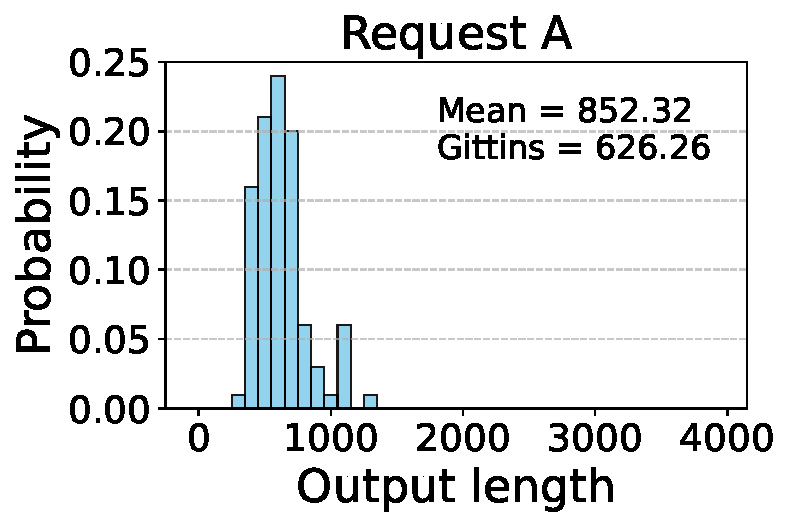
\includegraphics[width=0.45\linewidth]{figures/motivation_gittins_example_A.pdf}
        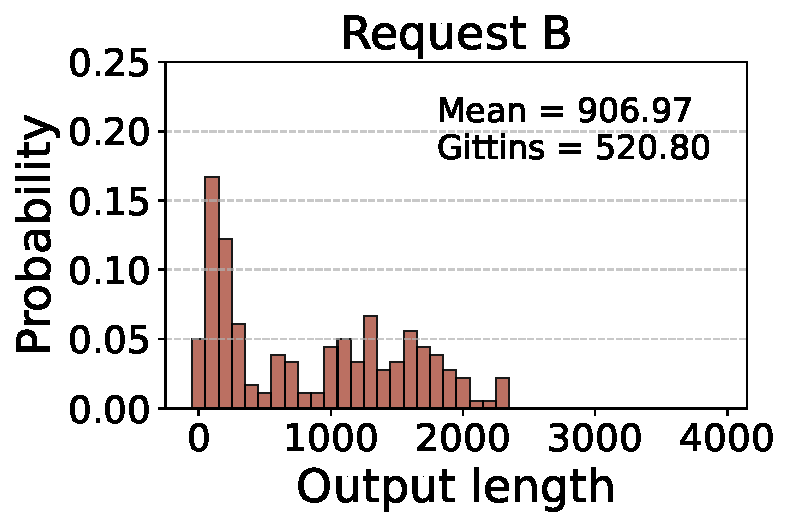
\includegraphics[width=0.45\linewidth]{figures/motivation_gittins_example_B.pdf}
    \caption{An example illustrating the deficiency of Mean-value-based request prioritization. While request-B has a larger Mean value, due to its irregular demand-distribution shape, however, serving it first can be expected to behave better in average TTLT.} % Mean Priority Determination under the Gittins Policy: despite a larger expected output length, request-2 has a smaller Gittins index due to higher near-term completion probability, and is thus prioritized by the Gittins policy.}
    \label{fig:gittins}
\end{figure}

In request queuing, we need to calculate a proper scheduling index out of each request's cost distribution (for which the mean value is not optimal, as suggested in Fig.~\ref{fig:gittins}).
In fact,  we notice that selecting a highest-priority inference to serve is similar to selecting the most-rewarding arm to take in a \emph{multi-armed bandit problem}~\cite{mahajan2008multi}: the cost distribution is essentially a reward distribution depicting how allocating additional resources to a request can help to yield inference completion. 
For such a multi-armed bandit problem with nondeterministic reward but deterministic reward distribution, in the literature it is known that the \emph{Gittins policy}~\cite{gittins1979bandit} can achieve the theoretically optimal performance.

Specifically, given a request with a cost distribution of $\mathcal{D}$, the Gittins policy calculates its Gittins index defined as $G(\mathcal{D})=\operatorname*{inf}_{\Delta>0,X\sim\mathcal{D}}{\frac{\operatorname{E}[\operatorname*{min}\{X,\Delta\}]}{\operatorname*{P}(X\leq\Delta)}}$; requests with smaller Gittins indices are prioritized in scheduling. % prioritizes the request with the shortest Gittins index in scheduling.
%then the Gittins policy prioritizes the request with the shortest Gittins index, which is defined as $G(D) = inf \delta > 0 and x\in D.
In that formula, $\operatorname{E}[\operatorname*{min}\{X,\Delta\}]$ represents the request service consumption when allocated a service budget $\Delta$, and $\operatorname*{P}(X\leq\Delta)$ represents its probability of successful completion before $\Delta$ is used up; $G$ thus represents the minimum amortized cost ever attainable for that request. 
It has been proven that, scheduling jobs based on such Gittins index (instead of the distribution expectation value) can yield the minimum average latency (TTLT)~\cite{gittins1989multiprocessor}. {The effect can be observed in Fig.~\ref{fig:gittins}, where the Gittins policy prioritizes the request that are more likely to complete in the near future.}
%Due to the theoretical optimality of the Gittins policy, we thus use Gittins index (instead of the mean output-length) as the request scheduling priority, which can yield the minimum average TTLT given their output-length distributions. 
%We thus use the Gittins index (instead of the mean output-length) as the scheduling priority, 
%In this way, in theory we can yield the minimum average inference completion time (TTLT) given their output-length distributions. 

Furthermore, the Gittins index of each pending request shall be properly updated at runtime after inference commencement.
As indicated by TRAIL~\cite{shahout2024don} and FastServe~\cite{wu2023fast}, enabling preemption is necessary to optimize the average TTLT (with negligible overheads given recent techniques like \emph{swap-compute overlapping} and \emph{KVCache prefetching}).  
Ideally, we need to keep refreshing the Gittins index of each active inference at runtime---with the information of \emph{remaining} service cost distribution.
Yet, continuously doing so after each inference step is still impractical---due to the high monitoring overhead as well as the thrashing risk (i.e., the relatively scheduling order of two requests with similar Gittins index may frequently reverse).
We therefore divide each request's cost range into multiple (defaulted to 10) buckets; the Gittins index of each request is refreshed only at bucket boundaries. 
In this way, we can seek a proper balance between rescheduling timeliness and system stability. 



